%%%%%%%%%%%%%%%%%%%%%%%%%%%%%%%%%%%%%%%%%%%%%%%%%%%%%%%%%%%%%%%%%%%%%%%%%%%%%
%%% LaTeX-Rahmen fuer das Erstellen von Masterarbeiten
%%%%%%%%%%%%%%%%%%%%%%%%%%%%%%%%%%%%%%%%%%%%%%%%%%%%%%%%%%%%%%%%%%%%%%%%%%%%%

%%%%%%%%%%%%%%%%%%%%%%%%%%%%%%%%%%%%%%%%%%%%%%%%%%%%%%%%%%%%%%%%%%%%%%%%%%%%%
%%% allgemeine Einstellungen
%%%%%%%%%%%%%%%%%%%%%%%%%%%%%%%%%%%%%%%%%%%%%%%%%%%%%%%%%%%%%%%%%%%%%%%%%%%%%
%!TeX spellcheck = en-GB
\documentclass[12pt,a4paper,twoside]{report}
\usepackage[utf8]{inputenc}

\usepackage{amsmath}
\usepackage[scaled=0.92]{helvet}
\usepackage[scaled=1.1]{nimbusmononarrow}
\usepackage[T1]{fontenc}
\usepackage{eurosym}
\usepackage[ngerman, english]{babel}
\usepackage{biblatex}
\addbibresource{Literature.bib}
\usepackage{csquotes}
\usepackage{microtype}
\usepackage{url}
\usepackage{graphics, graphicx}
\usepackage[margin=10pt,font=small,labelfont=bf]{caption}
\usepackage{sistyle}
\usepackage{latexsym}
\usepackage{hyperref}
\usepackage[textwidth=14cm,textheight=22cm,bindingoffset=6mm]{geometry}
\usepackage{wrapfig}

%\footskip 2cm
\parskip 0.5ex plus 0.1ex minus 0.1ex
%\parindent0pt


% Kann nach persönlichem Geschmack verändert werden.
\usepackage{fancyhdr}
\pagestyle{fancy}
\fancyhead[LO,RE]{\textsl{\nouppercase{\leftmark}}}
\fancyhead[LE,RO]{\thepage}
\fancyfoot{}

%\fancyhead[LE,RO]{\textsl{\rightmark}}


% Kommentar-Style zum Einfügen von To-Do's Befehle: \todo , \note und \listoftodos
\usepackage[textsize=footnotesize,textwidth=0.8in]{todonotes} % Kommentare einschalten
%\usepackage[disable]{todonotes} % Kommentarausgabe ausschalten
\setlength{\marginparwidth}{0.8in} % Abstand vom Rand
\newcommand{\note}{\todo[inline,color=yellow,caption={}]} %Notiz über volle Seitenbreite


\begin{document}

%%%%%%%%%%%%%%%%%%%%%%%%%%%%%%%%%%%%%%%%%%%%%%%%%%%%%%%%%%%%%%%%%%%%%%%%%%%%
%%% hier steht die neue Titelseite
%%%%%%%%%%%%%%%%%%%%%%%%%%%%%%%%%%%%%%%%%%%%%%%%%%%%%%%%%%%%%%%%%%%%%%%%%%%%

\begin{titlepage}
 \begin{center}
  {\LARGE Eberhard Karls Universität Tübingen}\\
  {\large Mathematisch-Naturwissenschaftliche Fakultät\\
  Fachbereich Informatik\\[2cm]}
  {\Huge\bf  MR-LINAC and CINE\\[1.5cm]}
{\Large\bf A viewing platform for 4d medical images with extensive labeling functionality\\[0.8cm]}
  {\Large Bachelorthesis Medical Informatics\\[3.0cm]}
  {\Large Henrike Sophie Weinmann}\\[0.5cm]
  Datum\\[3cm]
{\small\bf Marcel Früh}\\[1.0cm]
  \parbox{7cm}{\begin{center}{
  	\large Prof. Dr. rer. nat. Andreas Schilling}\\
	  Visual Computing\\
	  Fachbereich Informatik\\
	  Universität Tübingen
	  \end{center}}\hfill\parbox{7cm}{\begin{center}
  {\large Name Zweitgutachter}\\
	  Arbeitsbereich\\
	  Fachbereich Informatik\\
	  Universität Tübingen \end{center}
 }
  \end{center}
\end{titlepage}

%%%%%%%%%%%%%%%%%%%%%%%%%%%%%%%%%%%%%%%%%%%%%%%%%%%%%%%%%%%%%%%%%%%%%%%%%%%%
%%% Titelrückseite: Bibliographische Angaben
%%%%%%%%%%%%%%%%%%%%%%%%%%%%%%%%%%%%%%%%%%%%%%%%%%%%%%%%%%%%%%%%%%%%%%%%%%%%

\thispagestyle{empty}
\vspace*{\fill}
\begin{minipage}{11.2cm}
\textbf{Weinmann, Henrike:}\\
\emph{MR-LINAC and CINE, A viewing platform for 4d medical images with extensive labeling functionality}\\ Bachelorthesis Medical Informatics\\
Eberhard Karls Universit"at T"ubingen\\
Bearbeitungszeitraum: May 2021-bis
\end{minipage}
\newpage

%%%%%%%%%%%%%%%%%%%%%%%%%%%%%%%%%%%%%%%%%%%%%%%%%%%%%%%%%%%%%%%%%%%%%%%%%%%%

\pagenumbering{roman}
\setcounter{page}{1}

%%%%%%%%%%%%%%%%%%%%%%%%%%%%%%%%%%%%%%%%%%%%%%%%%%%%%%%%%%%%%%%%%%%%%%%%%%%%
%%% Seite I: Zusammenfassug, Danksagung
%%%%%%%%%%%%%%%%%%%%%%%%%%%%%%%%%%%%%%%%%%%%%%%%%%%%%%%%%%%%%%%%%%%%%%%%%%%%


\thispagestyle{plain}
\section*{Abstract}

MR guided radiotherapy has become a standard when treating cancer. The alternative to an operative removal of the tumor uses radiation, created by a linear accelerator (LINAC). MR-LINAC improves the accuracy of radiation by combining a LINAC with an MR imaging system. Magnetic resonance imaging (MRI) is optimal for viewing soft tissue such as most organs in the human body. It is also an important tool for detecting tumors in soft tissue such as the lungs and heart.
The CINE MRI technology makes it possible to observe a slice through a patient over a period of time.
This makes it easier to detect the margins of a structure and therefore decreases the risk of damaging tissue surrounding a tumor during treatment.
To be able to use those technologies to their full extent, a viewing platform is needed.
\newpage


\thispagestyle{plain}
\section*{Danksagung}

Hier kommen die Danksagungen hin (falls gewünscht)!!!

\newpage

%%%%%%%%%%%%%%%%%%%%%%%%%%%%%%%%%%%%%%%%%%%%%%%%%%%%%%%%%%%%%%%%%%%%%%%%%%%%%
%%% Erklaerung
%%%%%%%%%%%%%%%%%%%%%%%%%%%%%%%%%%%%%%%%%%%%%%%%%%%%%%%%%%%%%%%%%%%%%%%%%%%%%
\thispagestyle{empty}
\section*{Selbständigkeitserklärung}

%Hiermit versichere ich, dass ich die vorliegende Masterarbeit selbständig und nur mit den angegebenen Hilfsmitteln angefertigt habe und dass alle Stellen, die dem Wortlaut oder dem Sinne nach anderen Werken entnommen sind, durch Angaben von Quellen als Entlehnung kenntlich gemacht worden sind. Diese Masterarbeit wurde in gleicher oder ähnlicher Form in keinem anderen Studiengang als Prüfungsleistung vorgelegt.

% Erklärung aus dem Formular zur Anmeldung einer Bachelor-, Master- oder Diplomarbeit
% http://www.uni-tuebingen.de/fakultaeten/mathematisch-naturwissenschaftliche-fakultaet/fachbereiche/informatik/studium/downloads/allgemein-und-formulare.html
Hereby, I declare that I have composed the presented paper independently on my own and without any other resources than the ones indicated. All thoughts taken directly or indirectly from external sources are properly denoted as such.

This paper has neither been previously submitted to another authority nor has it been published yet.
\vskip 3cm

Place, Date	\hfill Signature \hfill

Hiermit erkläre ich, dass ich diese schriftliche Abschlussarbeit selbständig verfasst habe,
keine anderen als die angegebenen Hilfsmittel und Quellen benutzt habe und alle wörtlich
oder sinngemäß aus anderen Werken übernommenen Aussagen als solche gekennzeichnet
habe.
Datum, Ort, \hfill Unterschrift \hfill

\newpage
%%%%%%%%%%%%%%%%%%%%%%%%%%%%%%%%%%%%%%%%%%%%%%%%%%%%%%%%%%%%%%%%%%%%%%%%%%%%%
%%% Inhaltsverzeichnis
%%%%%%%%%%%%%%%%%%%%%%%%%%%%%%%%%%%%%%%%%%%%%%%%%%%%%%%%%%%%%%%%%%%%%%%%%%%%%

\renewcommand{\baselinestretch}{1.3}
\small\normalsize

\tableofcontents

\renewcommand{\baselinestretch}{1}
\small\normalsize

\newpage
\null
\thispagestyle{empty}
\newpage %%% Leerseite für Bindung, damit Content auf der rechten Seite anfängt

%%%%%%%%%%%%%%%%%%%%%%%%%%%%%%%%%%%%%%%%%%%%%%%%%%%%%%%%%%%%%%%%%%%%%%%%%%%%%
%%% Der Haupttext, ab hier mit arabischer Numerierung
%%% Mit \input{dateiname} werden die Datei `dateiname' eingebunden
%%%%%%%%%%%%%%%%%%%%%%%%%%%%%%%%%%%%%%%%%%%%%%%%%%%%%%%%%%%%%%%%%%%%%%%%%%%%%

\pagenumbering{arabic}
\setcounter{page}{1}

%% Introduction
%%%%%%%%%%%%%%%%%%%%%%%%%%%%%%%%%%%%%%%%%%%%%%%%%%%%%%%%%%%%%%%%%%%%
% Abstract
%%%%%%%%%%%%%%%%%%%%%%%%%%%%%%%%%%%%%%%%%%%%%%%%%%%%%%%%%%%%%%%%%%%%

\chapter{Introduction}\label{Introduction}
Viewing medical images on a light box is a thing of the past. In the digital age we're living in, tablets and monitors have taken over. With this change comes the need for new software. Mulitple applications for viewing X-Ray images, MR-scans, PET-scans etc. have already been developed. However, the digital world is evolving constantly and so existing applications need to be maintained, updated and improved. In recent times, machines have been so far improved, that 4d imaging is now possible. The fourth dimension being time. Those 4d scans are called CINE scans. CINE comes from the word cinematic and stands for the timely dimension which enables a filmlike view of the scanned area.
In the last few years Artificial Intelligence (AI) has made its way in to the medical field and is becoming more and more useful. These algorithms often work different as the human brain and so the outcome of the AI's calculations is usually the only useful information for the user.
In cooporation with Marcel Früh, I have developed a simplistic App for viewing the work of an AI that has been trained to calculate the movement of a point in a 4 dimensional dataset. Doctors still use markers and printed images to make plans for treatment or discuss a possible diagnosis with colleagues. Though this method requires a physical meeting, so it would become quite impossible when the coworker is a piece of software. Selections need to be made digitally and stored in such a way. that it is easily accessible to external software like an AI programm. The main goal was to create a tool that is easy to use and does not confuse the user with to many menu options and hidden features. In the following I will give a quick overview of medical image data and their purpose, as well as the current options for viewing 4d data. I will then explain my approach when designing and planning the app. 

\newpage

%%
%%%%%%%%%%%%%%%%%%%%%%%%%%%%%%%%%%%%%%%%%%%%%%%%%%%%%%%%%%%%%%%%%%%%
% Medical Data and imaging
%%%%%%%%%%%%%%%%%%%%%%%%%%%%%%%%%%%%%%%%%%%%%%%%%%%%%%%%%%%%%%%%%%%%
%!TeX spellcheck = en-GB
\chapter{Medical Data and imaging}
  \label{Medical Data and imaging}
\section{DICOM Format}
\begin{wrapfigure}{r}{0.3\textwidth}
    \vspace{-10pt}
   \centering
   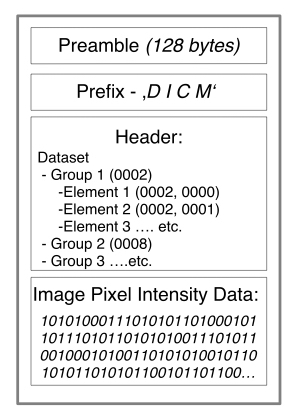
\includegraphics[width=0.28\textwidth]{figures/dicom.jpeg}
    \caption{structure of a DICOM file }
    \label{figure 2.1}
    \vspace{-15pt}
\end{wrapfigure}
DICOM  stands for Digital Imaging and Communications in Medicin. It provides standardized file format for images in medicine. Each DICOM file is made up of a header holding meta data and a body which contains the image. DICOM files tend to be fairly large, as they usually contain quite a few high resolution images. The meta data consists of a standardized series of tags which can be arranged in functional groups like "0010" patient information or "0008" study information.
DICOM images that are used for research or teaching are typically anonymized to protect the patients data. There are special programms to remove the according parts from the header.
Since DICOM files are not recognized as image files by most operating systems, including windows, macOS and ubuntu, they can only be viewed with the help of third-party software.
Thats why most equipment manufacturers either include a dicom viewer when the images are exported to a CD or just convert them to a JPEG, GIF or TIFF.
\cite{varmaManagingDICOMImages2012}
 \cite{ElsevierEnhancedReader}

  \section{Image Aquisition}
 \label{Image Aquisition}
 There are many different types of medical imaging. Each method has their own purpose and often more than one type of image is required to make a correct diagnosis. The first most common and also foundation for all other type of imaging techniques being an X-ray scan. It is on of the fastest methods to check for a bone fracture or tooth decay. However,  an X-ray don't have a depth of field therefore only show one view through the patients body. Hence sometimes an important detail can't be seen because it lies behind a less permeable material. PET Scans, CTs and MRI Scans give us the option to image the whole volume or a planar slice thorugh it. In the following I will give a quick summary on 2d, 3d and 4d datasets using the MRI scanning methodology as an example.

 \subsection{2d Slices}
  \label{2d Slice}
 In an MRI scanner a magnetic field is created, so that all protons in the patients body align themselfs with that field.
A 2d image is created by exciting a slice of tissue with a radio frequency (RF) impulse so that the protons in said tissue spin out of equilibrium.  and then detect the energy released when the protons in the tissue realign with the magnetic field.
\cite{MagneticResonanceImaging}
The thickness of the slices depend on the device used, but are normally between 2mm and 100mm.
\cite{johnson2DMultislice3D1999}
Modern machines are able to excite multiple slices of tissue, therefore making it possible to scan multiple slices at a time. This technique is called a 2D Multislice MRI.
\cite{vangeunsBasicPrinciplesMagnetic1999}

  \subsection{3d Volumetric imaging}
  \label{3d Volumetric imaging}
  There are two main ways to get a 3d image. One of these being a reconstruction of the original volume thorugh a collection of 2d slices. This sounds very simple, but there are actually may things to consider. Firstly, scantimes can be quite long, as there needs to be a short pause inbetween scans. Pictures need to be taken in the exact same position to avoid artifacts. Furthermore there will always be a space inbetween two slices. With methods such as the distance field interpolation, we have tools to overcome this proplem to a certain extent, but it will never be as exact as the second method of 3d imaging.
  \cite{vangeunsBasicPrinciplesMagnetic1999}
  Here, a whole slab of the volume gets excited.


  \subsection{4d medical imaging}
  \label{4d medical imaging}
  4d medical imaging is the process of generating multiple 3d images over time. It is an advanced imaging method, used to study a patients movements and observe changes. The human body naturally moves at all times. Respiratory and cardiac motion, as well as digestion and muscle movements, cause the movement of surrounding tissues. It has always been a challenge to capture these movements in 3d medical images or get an image in a good position to see a certain feature. With 4d imaging, medical professionals are able to capture the whole movement and pick the best time frames for their issue.

\section{Image-guided therapy}
\label{Image-guided therapy}

\subsection{planning}
  \label{planning}
When planning an operation or radiation session, MRI is mainly used for gross tumor volume (GTV) and organs at risk (OAR) delineation.
\cite{lineyMRIRadiotherapyPlanning2019}

  \subsection{radiotherapy and LINAC}
    \label{radiotherapy and LINAC}
stereotactic radiosurgery (SRS)

\newpage

%%
%%%%%%%%%%%%%%%%%%%%%%%%%%%%%%%%%%%%%%%%%%%%%%%%%%%%%%%%%%%%%%%%%%%%
% State of the art
%%%%%%%%%%%%%%%%%%%%%%%%%%%%%%%%%%%%%%%%%%%%%%%%%%%%%%%%%%%%%%%%%%%%

\chapter{State of the art}
  \label{SOTA}
\section{Viewers for medical images}
\subsection{proprietary DICOM viewers}
Many scan machines today are connected to a Picture Archiving and Communication System (PACS). If not, the manufacturers usually provide a viewer in form of a standalone PC. The viewing software often comes with a variety of tools such as 3d reconstruction and rendering of multiplanar scans. Furthermore they give the option to export the DICOM file as png or jpeg, so they can be viewed on a normal PC by patients. \cite{ElsevierEnhancedReader}

\subsection{Third party DICOM viewers}
\label{Third party DICOM viewers}
When searching for a DICOM viewer online, one will find a plethora of options. They range from simple viewers which just display the image to high class applications useful for teaching, research and even as mini-PACS. Still, there is no piece of software that does it all. Most Viewers specialize as the enquiry for them is constantly evolving.
\cite{varmaFreeDICOMBrowsers2008}

\section{Image labeling  and editing Software}
\label{Image labeling and editing Software}
Editing software can be quite expensive. Depending on the functionality and features provieded prices change. One of the best and wellknown photo editing software being Adobe's Photoshop. After importing an image as DICOM, jpeg, png etc. pretty much all alterations imaginable can be made. Just like with the viewing software, there are lots of free options downloadable from the internet. Most of these however, only give selected options for editing.
A very common edit, useful for teaching or specification in publlications, is the use of red arrows. These can even be added in Powerpoint or Paint.

\subsection{Segmentation}
\label{Segmentation}
In IGRT segmentation of a tumor is one of the crucial parts of planning a radiation session. A to small segmentation could leave vital parts of the tumor and therefore be less effective, while a segmentation that is to large will hurt the surrounding tissue.
As an approach to help optimize the segmentation process semi-autumatic as well as fully automated selection tools have appeard.
\cite{heckelSketchBasedEditingTools2013}

\newpage

%%
%%%%%%%%%%%%%%%%%%%%%%%%%%%%%%%%%%%%%%%%%%%%%%%%%%%%%%%%%%%%%%%%%%%%
% Concept
%%%%%%%%%%%%%%%%%%%%%%%%%%%%%%%%%%%%%%%%%%%%%%%%%%%%%%%%%%%%%%%%%%%%

\chapter{A viewing platform for 4d image data}
  \label{A viewing platform for 4d image data}
  \section{Goal}
  The goal of this project, was to develop a viewing platform for MRI CINE data, which is easy to use and still provides useful editing and labeling tools. The focus was set on the labeling funcionality of the app which is supposed to give the user the option to mark ceratin places or areas. The app should be intuitively usable without a tutorial or a long learning phase. Given that most medical applications don't look very appealing, it also became a personal goal of mine to make this application look nice as well.

\section{original approach}
\label{original approach}
To build the user interface I ended up using PyQt, as it works nicely with the other python modules in use. However, the first versions of the application's GUI were using a combination of VTK and PyQt. In these versions all user input was handeled by VTK which is a very powerful tool but doesn't necessarily work well together with the PyQt part of the app. Especially the newer versions of VTK and PyQt in conjunction caused more and more problems for me. After some thought, I decided to limit this project to 2d selections only, thus there was no need for a 3D Module anymore and I ended up using Matplotlib instead.


\subsection{Loading data into the app}
\label{Loading data into the app}
To be able to view a data set, it first must be loaded into the app. My first approach was to load a folder via pathname, as no libraries or extra packages would be needed for that. However this method was not very userfriendly, because a single typo would lead to an error message. The solution was to open a directory or file with help of the os beneath. This was way more intuitive and also gave me the option to specify which kinds of data should be allowed to open. Although I had already checked for the correct suffix in the path, the QFileDialog Class had a useful feature that prevented the user from trying to open an unsuitable dataset.
Since the main focus was to display CINE datasets, each set consistet of multiple slices and a number of different timesteps for each slice. To have full accesssiblity to the whole dataset at all times during the editing process, the first step was to load all image parts of the DICOM files into a multidimensional array.

\subsection{Displaying the DICOM images}
\label{Displaying the DICOM images}
\paragraph{Media bar}
If the loaded data set were to contain multiple images in a folder, the app recognizes them as a CINE sequence and provides a media bar with the options to play the video or go through it frame by frame.
This option is automatically removed when only a single image or only one image per slice ist provided.

\section{Labeling}
\label{Labeling}
\paragraph{single point selection}
\paragraph{multiple point selection}

\subsection{Polygonal segmentation}
\label{Polygonal segmentation}
To make a 'multi point selection' better visible and also give the user the option to select an area rather than specific points, the option for polygonal segmentation was added.

\subsection{Editing}
\label{Editing}
There are five main editing funcionalities. They don't alter the original image, but change how it is displayed as well as give the option to make changes.
\paragraph{specify color map}
There are several different color maps available. The standard when opening the app being 'bone', which resembles the original look of an X-ray film. I chose this color map a the standard because most people will be used to the look. Still, it might not be the best option for some usecases which is why the option to chose another one exists.
\paragraph{edit labeling}
As mentioned before, the user is able to make selections on the image. Sometimes a selection needs to be moved or completly deleted. There are a few different options available.
\begin{itemize}
    \item Clear all selections
    \item Erase a specific selection
    \item Move a selection
\end{itemize}
 \paragraph{change contrast}
 There are two ways to change the contrast. For a new user the slider in the image editing menu might be the most intuitive. However quite a few image viewers give the option to change the contrast via mouse as well. Although my intention was not to have any hidden features, this one was an exception since it is fairly established.
\paragraph{export and save}
The 'export and save' function allows the user to save the current figure with all selections made to their computer.
\paragraph{hide selections}
This fuction was needed to be able to quickly check the original image without loosing the already made selections. It also allows to save 2 Versions of the displayed image. One with selections and one without.
\section{Design}
\label{Design}
Most applications have a very bland design and purely focus on usability. Since some of these apps are very old, the design of them doesn't match what some users might be used to from modern apps and therefore even hinder their usability. They can be very cluttered with no sense of hirarchy as to what is important for the user and what feature will only be useful every once in a while.

\subsection{Layout of the application}
\label{Layout of the application}
When designing the app, I had a very modular style in mind. This way, it would be easy to add on to the existing app or simplify if needed. The main portion of the app would be the DICOM viewer, since it would be what needs to be displayed the largest in order to be useful.

\subsection{Simplicity}
\label{Simplicity}
\paragraph{color palette}
In order to avoid to many clashing collors, I crated a monochromatic color palette. By using greys and blues of different saturation and brightness values the contrast between different texts and their background would still be given.

\paragraph{logos}
All logos and buttons were designed by me to avoid any copyright issues. I tryed to match the rest of the application with rounded edges and matching colors.

\newpage

%%
%%%%%%%%%%%%%%%%%%%%%%%%%%%%%%%%%%%%%%%%%%%%%%%%%%%%%%%%%%%%%%%%%%%%
% Evaluation
%%%%%%%%%%%%%%%%%%%%%%%%%%%%%%%%%%%%%%%%%%%%%%%%%%%%%%%%%%%%%%%%%%%%

\chapter{Evaluation}
  \label{Evaluation}

BlaBlaBla

\newpage

%%
%%%%%%%%%%%%%%%%%%%%%%%%%%%%%%%%%%%%%%%%%%%%%%%%%%%%%%%%%%%%%%%%%%%%
% Recapitulation and Future
%%%%%%%%%%%%%%%%%%%%%%%%%%%%%%%%%%%%%%%%%%%%%%%%%%%%%%%%%%%%%%%%%%%%

\chapter{Recapitulation and Future possibilities}
  \label{Recapitulation and Future possibilities }

BlaBlaBla

\newpage

%%%%%%%%%%%%%%%%%%%%%%%%%%%%%%%%%%%%%%%%%%%%%%%%%%%%%%%%%%%%%%%%%%%%%%%%%%%%%
%%% Bibliographie
%%%%%%%%%%%%%%%%%%%%%%%%%%%%%%%%%%%%%%%%%%%%%%%%%%%%%%%%%%%%%%%%%%%%%%%%%%%%%
\setcounter{biburllcpenalty}{9000}
\setcounter{biburlucpenalty}{9000}
\setcounter{biburlnumpenalty}{9000}
\addcontentsline{toc}{chapter}{Sources}
\printbibliography


%% Verwende jetzt Biblatex.

\newpage
\appendix
%%%%%%%%%%%%%%%%%%%%%%%%%%%%%%%%%%%%%%%%%%%%%%%%%%%%%%%%%%%%%%%%%%%%%%%%%%%%%
%%% Abk"urzungsverzeichnis
%%%%%%%%%%%%%%%%%%%%%%%%%%%%%%%%%%%%%%%%%%%%%%%%%%%%%%%%%%%%%%%%%%%%%%%%%%%%%

\addcontentsline{toc}{chapter}{List of abbreviations}
\chapter*{List of abbreviations}

\begin{tabbing}
	\textbf{FACTOTUM}\hspace{1cm}\=Schrott\kill
    \textbf{AI}\>Artificial intelligence  \\
	\textbf{LINAC}\>Linear accelerator \\
    \textbf{IGRT}\>Image guided radiotherapy  \\
	\textbf{MRI} \> Magnetic Resonance Imaging\\
    \textbf{RF} \> Radio Frequency\\
    \textbf{PACS} \> Picture Archiving and Communication System\\
    \textbf{SRS} \> Stereotactic radiosurgery\\
    \textbf{GTV} \> Gross tumor volume\\
    \textbf{OAR} \> Organs at risk\\
    \textbf{ROI} \> Region of interest\\
    \textbf{VC-MRI} \> Volumetric CINE Magnetic Resonance Imaging\\
\end{tabbing}

\newpage

%%%%%%%%%%%%%%%%%%%%%%%%%%%%%%%%%%%%%%%%%%%%%%%%%%%%%%%%%%%%%%%%%%%%%%%%%%%%%
%%% Abbildungsverzeichnis
%%%%%%%%%%%%%%%%%%%%%%%%%%%%%%%%%%%%%%%%%%%%%%%%%%%%%%%%%%%%%%%%%%%%%%%%%%%%%

\renewcommand{\baselinestretch}{1.3}
\small\normalsize

\addcontentsline{toc}{chapter}{List of images}
\listoffigures

\renewcommand{\baselinestretch}{1}
\small\normalsize

\newpage

%%%%%%%%%%%%%%%%%%%%%%%%%%%%%%%%%%%%%%%%%%%%%%%%%%%%%%%%%%%%%%%%%%%%%%%%%%%%%
%%% Tabellenverzeichnis
%%%%%%%%%%%%%%%%%%%%%%%%%%%%%%%%%%%%%%%%%%%%%%%%%%%%%%%%%%%%%%%%%%%%%%%%%%%%%

\renewcommand{\baselinestretch}{1.3}
\small\normalsize

\addcontentsline{toc}{chapter}{List of tables}
\listoftables

\renewcommand{\baselinestretch}{1}
\small\normalsize

\newpage

%%%%%%%%%%%%%%%%%%%%%%%%%%%%%%%%%%%%%%%%%%%%%%%%%%%%%%%%%%%%%%%%%%%%%%%%%%%%%
%%% End
%%%%%%%%%%%%%%%%%%%%%%%%%%%%%%%%%%%%%%%%%%%%%%%%%%%%%%%%%%%%%%%%%%%%%%%%%%%%%

\end{document}
